\section{领域泛化}
我们从最基础的泛化形式开始，即OPD的训练和评估均处于同一领域（数学）但其分布不同。我们首先探讨训练问题的难度（通过教师和学生的通过率衡量）是否影响OPD在该领域的泛化能力（第~\ref{subsec:difficulty}节）。接着，我们研究在英文数学问题上获得的能力是否能泛化到中文问题和更长时序的问题，以及模型原点如何塑造这些行为（第~\ref{subsec:lang_horizon}节）。

\subsection{训练问题难度}
\label{subsec:difficulty}
我们从两个方面衡量问题的难度：\textbf{\emph{教师}的通过率}，这是训练前即可获得的固定难度估计；以及 \textbf{\emph{学生}的通过率}，这是一个在训练过程中动态变化的信号。
\paragraph{教师通过率。}
为研究教师端通过率（teacher-end pass-rate）对 OPD 在领域内泛化能力的影响，我们针对每个 BigMath 问题采样四个教师响应，并构建三个各含 25K 个问题的子集：\textbf{简单}（通过率 $=1$）、\textbf{困难}（通过率 $=0$）和 \textbf{随机}（从全部问题中随机采样），其余条件均保持不变。如图~\ref{fig:teacher_pass_rate_combined} 所示，这三个子集在所有教师–学生组合上最终收敛至几乎相同的准确率。这表明：\emph{\textbf{OPD 教授学生模型的是教师的推理模式，而非特定问题的正确答案}}，因此即使教师无法端到端地解决某问题，仍可为其提供具有信息量的 token 级监督~\cite{chandra2025shape}。  
我们还在极简单问题（小学数学 GSM8K）和极困难问题（DeepMath-103K 中最难的子集）上开展了实验，得到了类似结论：在这些数据上训练仍能恢复默认 BigMath-随机设置下 OPD 增益的 $80\%$ 以上（附录~\ref{sec:appendix_add_results} 中图~\ref{fig:extreme_difficulty}）。因此，按难度对教师端数据进行筛选影响甚微。  
\begin{insightbox}  
\textbf{核心结论：}  
OPD 传递的是教师的\emph{推理行为}，而非其对特定问题的答案。在数学领域内，以教师通过率为指标衡量的训练问题难度，对领域内泛化能力影响甚小：教师从未解决过的问题与始终能解决的问题同样有效；甚至小学数学问题亦能恢复大部分 OPD 增益。  
\end{insightbox}
\begin{figure*}[t]
    \centering
    \begin{subfigure}[b]{0.32\linewidth}
        \centering
        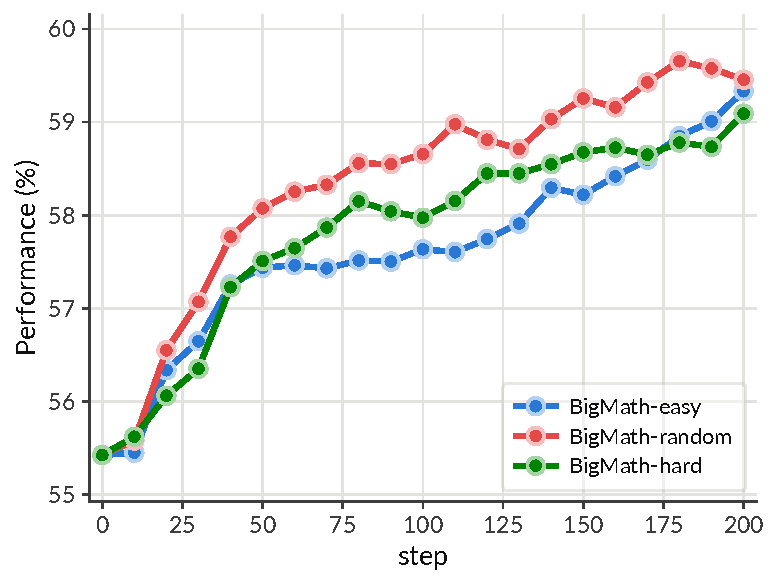
\includegraphics[width=\linewidth]{latex/figures/findings_1/teacher_pass_rate/32b_to_8b_math_teacher_pass_rate_mainmath6_avg.pdf}
        \caption{Qwen3-32B $\rightarrow$  Qwen3-8B-SFT}
        \label{fig:teacher_pass_32b_to_8b}
    \end{subfigure}
    \hfill
    \begin{subfigure}[b]{0.32\linewidth}
        \centering
        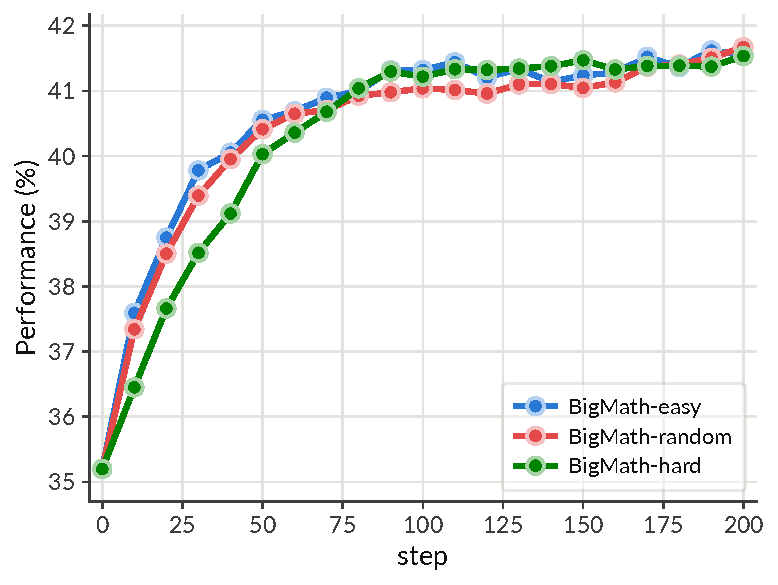
\includegraphics[width=\linewidth]{latex/figures/findings_1/teacher_pass_rate/7b_to_1d5b_math_teacher_pass_rate_mainmath6_avg.pdf}
        \caption{Polaris-7B $\rightarrow$ DS-distill-1.5B}
        \label{fig:teacher_pass_7b_to_1d5b}
    \end{subfigure}
    \hfill
    \begin{subfigure}[b]{0.32\linewidth}
        \centering
        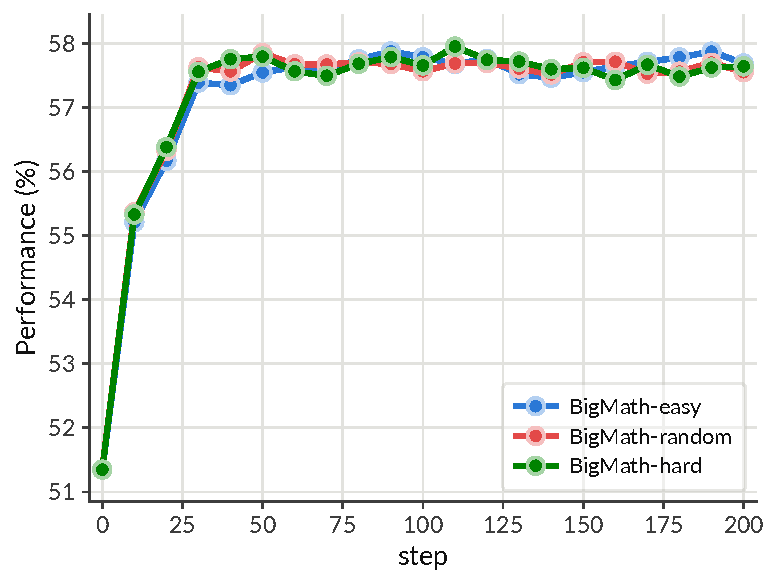
\includegraphics[width=\linewidth]{latex/figures/findings_1/teacher_pass_rate/7b_to_7b_math_teacher_pass_rate_mainmath6_avg.pdf}
        \caption{Polaris-7B $\rightarrow$ DS-distill-7B}
        \label{fig:teacher_pass_7b_to_7b}
    \end{subfigure}

    \caption{领域内数学准确率（六项英文基准的平均值）对训练问题的难度不敏感，该难度由教师模型的通过率衡量。每个图表比较了三个BigMath子集：\textbf{简单}（通过率 $=1$ ，教师解决全部四个回溯），\textbf{困难}（通过率 $=0$ ，教师一个也未解决），以及 \textbf{随机}（从整个数据集中随机采样）。这三个子集在所有教师-学生组合下最终准确率均收敛至几乎相同水平。}
    \label{fig:teacher_pass_rate_combined}
\end{figure*}
\begin{table*}[htbp]
\centering
\caption{OPD 在六项数学基准上的泛化性能，采用学生端动态采样。仅丢弃学生已解决的问题（通过率 $\in[0,1)$）时，平均性能最佳。绿色/红色标记表示相对于无动态采样基准的每项基准性能提升/下降。}
\label{tab:pass-rate-eval}
\resizebox{\textwidth}{!}{%
\begin{tabular}{c|cccccc|c}
\toprule
\textbf{Filtering Strategy} & \textbf{AMC2023} & \textbf{MATH500} & \textbf{AIME2025} & \textbf{AIME2026} & \textbf{BeyondAIME} & \textbf{OlymMATH-Hard} & \textbf{Average} \\
\midrule
\midrule
\multicolumn{8}{c}{\textbf{\textit{Teacher: Polaris-7B, Student: DS-distill-1.5B}}} \\
\midrule
\textbf{w/o dynamic sampling} & $80.4\%$ & $89.5\%$ & $30.2\%$ & $30.1\%$ & $13.6\%$ & $4.7\%$ & $41.4\%$ \\
\midrule
\textbf{pass-rate} $\mathbf{= 0}$        & \cellcolor{red!25}$78.8\%$ & \cellcolor{green!25}$90.1\%$ & \cellcolor{green!25}$30.5\%$ & \cellcolor{red!25}$30.0\%$ & \cellcolor{green!25}$14.7\%$ & \cellcolor{red!25}$4.4\%$ & $41.4\%$ \\
\textbf{pass-rate} $\mathbf{= 1}$        & \cellcolor{red!25}$79.9\%$ & \cellcolor{green!25}$89.7\%$ & \cellcolor{green!25}$30.9\%$ & \cellcolor{red!25}$28.9\%$ & \cellcolor{green!25}$14.7\%$ & \cellcolor{red!25}$4.0\%$ & $41.4\%$ \\
\textbf{pass-rate} $\mathbf{\in [0, 1)}$ & \cellcolor{green!25}$80.9\%$ & \cellcolor{green!25}$89.8\%$ & \cellcolor{green!25}$31.2\%$ & \cellcolor{green!25}$31.1\%$ & \cellcolor{green!25}$13.7\%$ & \cellcolor{green!25}$5.4\%$ & $\mathbf{42.0}\%${\footnotesize \textcolor{green!60!black}{(\textbf{+0.6 pp})}} \\
\midrule
\midrule
\multicolumn{8}{c}{\textbf{\textit{Teacher: Light-R1-14B, Student: DS-distill-7B}}} \\
\midrule
\textbf{w.o. dynamic sampling} & $91.7\%$ & $95.0\%$ & $42.8\%$ & $49.7\%$ & $26.5\%$ & $8.7\%$ & $52.4\%$ \\
\midrule
\textbf{pass-rate} $\mathbf{= 0}$        & \cellcolor{green!25}$92.1\%$ & \cellcolor{red!25}$94.3\%$ & \cellcolor{red!25}$40.2\%$ & \cellcolor{green!25}$50.3\%$ & \cellcolor{green!25}$28.2\%$ & \cellcolor{red!25}$7.8\%$ & $52.1\%${\footnotesize \textcolor{red!60!black}{(\textbf{-0.3 pp})}} \\
\textbf{pass-rate} $\mathbf{= 1}$        & \cellcolor{green!25}$92.3\%$ & \cellcolor{red!25}$94.5\%$ & \cellcolor{red!25}$42.2\%$ & \cellcolor{red!25}$48.7\%$ & \cellcolor{green!25}$28.0\%$ & \cellcolor{red!25}$8.0\%$ & $52.2\%${\footnotesize \textcolor{red!60!black}{(\textbf{-0.2 pp})}} \\
\textbf{pass-rate} $\mathbf{\in [0, 1)}$ & \cellcolor{green!25}$92.1\%$ & \cellcolor{green!25}$95.4\%$ & \cellcolor{green!25}$43.2\%$ & \cellcolor{green!25}$50.6\%$ & \cellcolor{green!25}$28.0\%$ & \cellcolor{red!25}$7.5\%$ & $\mathbf{52.8}\%${\footnotesize \textcolor{green!60!black}{(\textbf{+0.4 pp})}} \\
\bottomrule
\end{tabular}%
}
\end{table*}

\paragraph{学生通过率。}
我们在 BigMath 的随机子集上测试了两组模型：Polaris-7B\,$\rightarrow$ \,DS-distill-1.5B 和 Light-R1-14B\,$\rightarrow$ \,DS-distill-7B。  
对每个问题，我们采样四个学生响应，并将三种策略与无过滤基准（no-filtering baseline）进行比较：仅保留完全未解出的问题（通过率 $=0$ ）、仅保留完全解出的问题（通过率 $=1$ ），或仅丢弃完全解出的问题（通过率 $\in[0,1)$ ）。如表~\ref{tab:pass-rate-eval} 所示，限制于任一极端情形均无益处；而 \emph{\textbf{动态丢弃学生已能完全解出的问题，则为两组模型均带来微小但稳定的提升}}。该结果符合直觉：一旦学生能够稳定地解出某问题，教师便不应继续在该问题上对其推理过程进行重新对齐。综上，OPD 在领域内的泛化能力在很大程度上不受训练问题难度的影响。
\begin{insightbox}
\textbf{要点：}
动态丢弃学生已能完全解出的问题（即通过率 = 0）可带来微小但稳定的改进，表明教师不应持续对已掌握推理能力的学生进行重新对齐。
\end{insightbox}
\subsection{跨语言与推理范围的泛化}
\label{subsec:lang_horizon}

\begin{figure*}[t]
    \centering

    \begin{subfigure}[b]{0.99\linewidth}
        \centering
        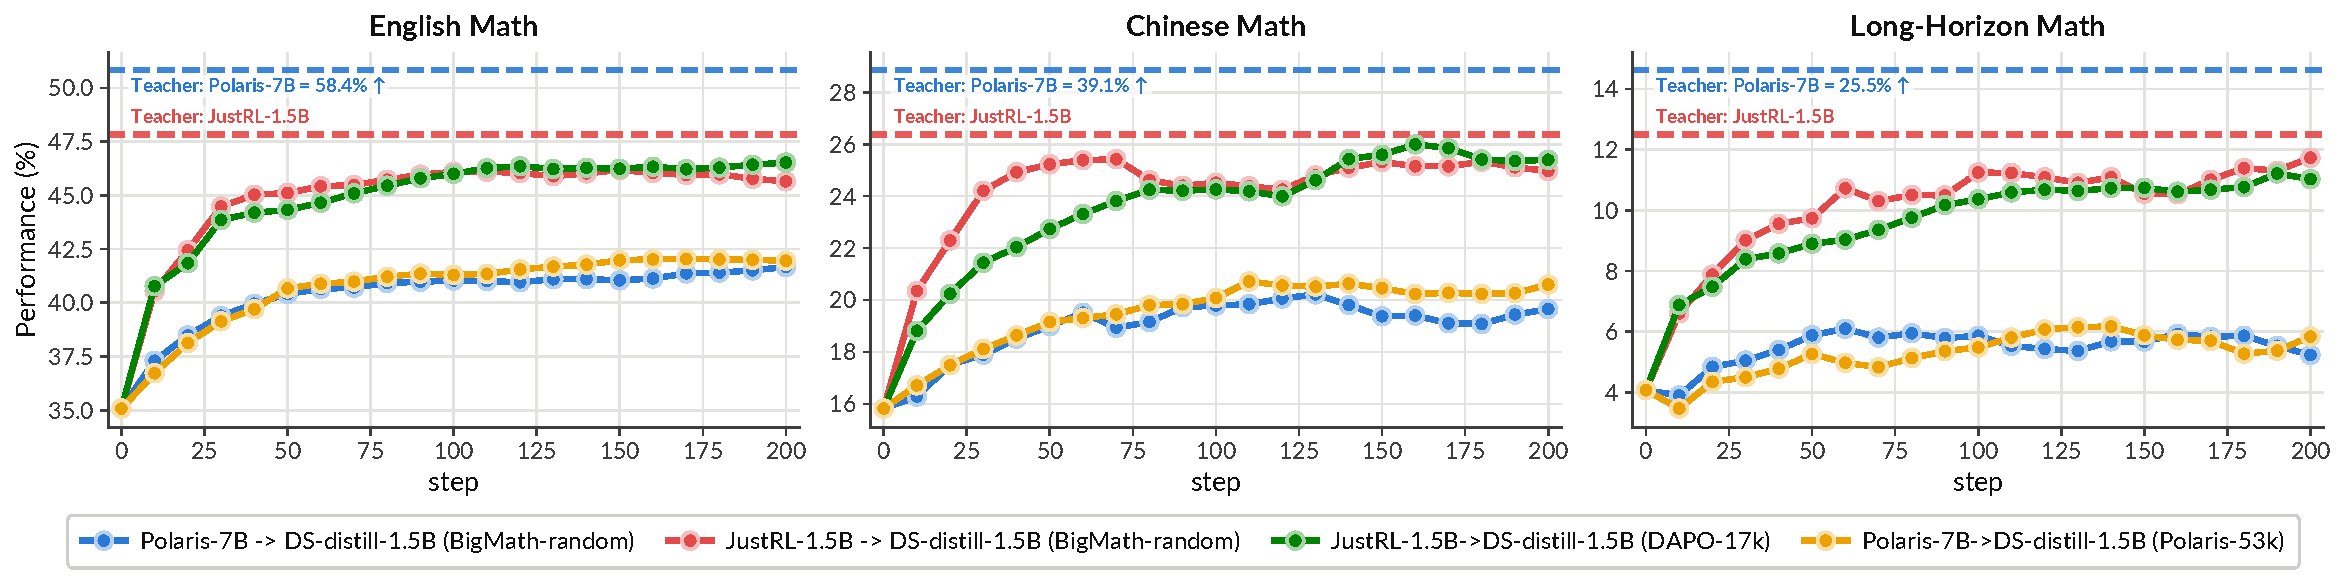
\includegraphics[width=\linewidth]{latex/figures/findings_1/1d5b_same_different_source_comparison_math_math_panel.pdf}
        \caption{DS-蒸馏-1.5B}
        \label{fig:1d5b_cross_language_horizon}
    \end{subfigure}

    \begin{subfigure}[b]{0.99\linewidth}
        \centering
        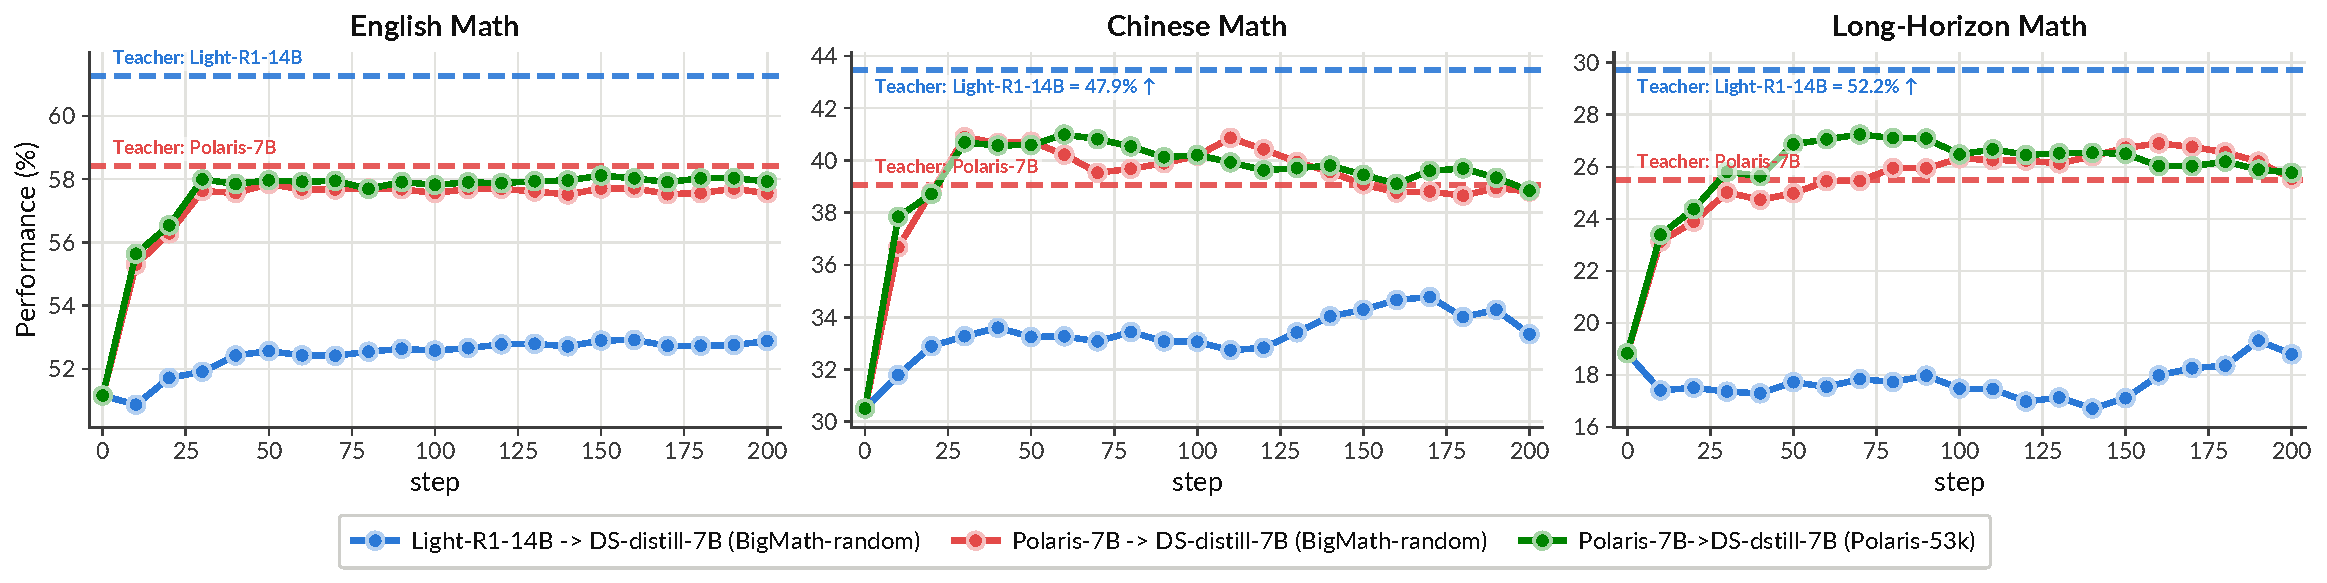
\includegraphics[width=\linewidth]{latex/figures/findings_1/7b_same_different_source_comparison_math_math_panel.pdf}
        \caption{DS-蒸馏-7B}
        \label{fig:7b_cross_language_horizon}
    \end{subfigure}

    \caption{OPD仅在英文数学题上训练，但能泛化到中文和长时程数学基准测试，然而收益的大小和稳定性取决于模型来源。每个图表中，同一学生配对了同源和跨源的教师；虚线标记了教师的准确率。}
    \label{fig:cross_language_and_horizon_same_different_origin}
\end{figure*}

我们探讨所获得的推理能力是否能泛化到两种偏移分布上：(1) 训练数据为英文数学题，而评估数据为中文数学题；(2) 训练问题原本是原子性的且短时域的，而评估问题为长时域~\citep{dziri2023faith, shojaee2025the,lu2025r}，由\emph{多个数学问题组合而成}；这考察了系统性泛化能力。我们评估两名学生，DS-distill-1.5B/7B，每名学生分别配对一个同源教师和一个跨源教师，所有模型均在BigMath-random上进行训练。图~\ref{fig:cross_language_and_horizon_same_different_origin}显示，\emph{\textbf{OPD不仅提升了分布内英文数学题的表现，还提升了中文和长时域分布的表现}}。仅在英文数据上训练即可提升中文数学题的准确率，说明所获得的能力并不依赖于训练问题的表面语言；在长时域基准上也出现了性能提升，这些题目需要长时域推理以及在子问题间传递中间答案，而这种结构在训练数据中并不存在。然而，同源教师与跨源教师之间的性能提升幅度存在显著差异，我们将在下文进一步分析。

\paragraph{模型原点的作用。}
\label{subsec:origin_indomain}
对于每个学生，我们在图~\ref{fig:cross_language_and_horizon_same_different_origin} 中比较了在同源教师与跨源教师下的 OPD 泛化表现（例如，对于 DS-distill-1.5B，JustRL-1.5B 是同源教师，而 Polaris-7B 是跨源教师）。有两个观察尤为突出。  
首先，\emph{\textbf{更强的教师并不意味着更强的学生：同源教师远比跨源教师更有效}}。例如，在 7B 面板中，跨源的 Light-R1-14B 在独立评估中的准确率明显高于同源的 Polaris-7B（虚线），但其生成的学生模型却弱得多，并且在长推理链数学任务上，跨源学生模型相较于初始模型几乎没有任何显著提升。其次，\emph{\textbf{同源 OPD 能使学生模型始终接近教师的准确率，这一点不仅体现在分布内英文评估中，也适用于语言和推理长度的分布外情况}}。一个合理的解释是，原点可作为教师策略与学生之间兼容性的一个指示器，因此 \emph{\textbf{同源配对能够整体对齐，并将这种对齐能力跨分布传递}}。  
此外，实证结果还表明，使用教师的 RL 训练提示（例如，Polaris-7B 使用 Polaris-53k，JustRL-1.5B 使用 DAPO-17k）在 OPD 性能上并未带来显著差异。

\begin{insightbox}
\textbf{要点：}
OPD 也能在领域内分布变化的情况下工作，但主要是在同一原点情景下：仅在英语、短时程数学上训练的学生，在拥有同一原点教师时，能够在中文和长时程数学上接近教师的水平，而拥有跨原点教师（即使其表现优于同一原点教师）时，提升幅度较小。
\end{insightbox}
